\documentclass[10pt,a4paper,twocolumn]{article}
\usepackage[T1]{fontenc}
\usepackage[utf8]{inputenc}
\usepackage{newtxtext,newtxmath}
\usepackage[margin=1.8cm,columnsep=0.7cm]{geometry}
\usepackage{graphicx,booktabs,array,amsmath,microtype}
\usepackage[super,sort&compress]{natbib}
\usepackage{xcolor}
\usepackage[normalem]{ulem}
\usepackage{xurl,xr-hyper}
\usepackage[colorlinks=true,allcolors=teal]{hyperref}

\usepackage{authblk}







\externaldocument[esi-]{esi-build/supplementary_information}[supplementary_information.pdf]
\setlength{\parindent}{1em}
\setlength{\parskip}{0pt}
\newcommand{\CPtwoK}{CP2K}
\newcommand{\Skala}{Skala}
\newcommand{\GPW}{GPW}
\newcommand{\GAPW}{GAPW}
\newcommand{\GTH}{GTH}
\newcommand{\GX}{GAPW-XC}
\newcommand{\uvec}{\boldsymbol{u}}
\newcommand{\gvec}{\boldsymbol{g}}
\title{Native implementation of the machine-learned Skala exchange--correlation functional in CP2K: Unified one-centre reconstruction for molecular and condensed-phase calculations}
\author[1,2]{Johann Pototschnig}
\author[1,2]{Franz P\"oschel}
\author[3]{J\"urg Hutter}
\author[1,2,4]{Thomas D. K\"uhne\textsuperscript{\dag}}
\affil[1]{Center for Advanced Systems Understanding (CASUS), G\"orlitz, Germany}
\affil[2]{Helmholtz-Zentrum Dresden-Rossendorf, Dresden, Germany}
\affil[3]{Department of Chemistry, University of Zurich, Zurich, Switzerland}
\affil[4]{Institute of Artificial Intelligence, Technische Universit\"at Dresden, Dresden, Germany}
\date{}
\graphicspath{{figures/}}
\begin{document}
\raggedbottom
\twocolumn[\maketitle
\begin{center}\small
\textsuperscript{\dag}E-mail: \href{mailto:tkuehne@cp2k.org}{tkuehne@cp2k.org}
\end{center}
\begin{abstract}
Machine-learned exchange--correlation (XC) functionals combine high molecular accuracy with the prospect of efficient condensed-phase simulation. We implement the Skala XC functional natively in CP2K using its Gaussian and plane-wave (GPW) and Gaussian and augmented-plane-wave (GAPW) methods. The central development is a joint one-centre reconstruction of density, density gradients, and kinetic-energy density before functional evaluation. This preserves mixed gradient terms and nonlocal couplings across the smooth and atom-local contributions for all-electron and pseudopotential calculations. The XC-specific GAPW representation resolves rapidly varying local contributions on atom-centred grids, reducing the required plane-wave resolution for pseudopotential calculations as well. The implementation incorporates Brillouin-zone sampling and point-group symmetry reduction.
With sufficiently flexible orbital bases, the native implementation retains the molecular benchmark accuracy of our earlier GauXC formulation. Crystalline CO$_2$, NH$_3$, and urea probe complementary interaction regimes, ranging from dispersion and quadrupolar electrostatics to hydrogen bonding and cooperative hydrogen-bond networks. All-electron Skala--D3(BJ) calculations give a mean absolute error of 1.54~kJ~mol$^{-1}$ against diffusion Monte Carlo for this three-crystal set. Across all thirteen DMC-ICE13 phases, the corresponding errors are 1.16~kJ~mol$^{-1}$ for absolute lattice energies and 0.82~kJ~mol$^{-1}$ for the twelve relative energies to ice Ih. At fixed experimental geometries, the all-electron/mixed-core calculations yield a band-gap MAE of 0.43~eV on the 15-material comparison set, substantially lower than those of commonly used semilocal functionals and comparable to those of widely used hybrid functionals. The LC10 benchmark nevertheless reveals systematically underestimated equilibrium lattice constants, indicating structural overbinding.  The resulting framework connects molecular Skala to condensed-phase electronic structure and enables future development using periodic many-body reference data.
\end{abstract}
\vspace{0.5cm}]

\section{Introduction}

The accuracy of Kohn--Sham density-functional theory (DFT) is governed to a large extent by the approximation to the exchange--correlation (XC) functional.\cite{Kohn1999Nobel,Jones2015DFT} Learning this contribution from accurate electronic-structure data offers an alternative to conventional functional forms, as exemplified by the DM21 functional.\cite{Kirkpatrick2021DM21} Skala combines local density information with a learned nonlocal representation and has demonstrated strong performance across molecular energetics.\cite{Skala2025} The Skala-1.1 model used here was trained on molecular and atomic data, with no periodic electron densities in its reported training set.\cite{Skala2025,Ehlert2026ACC} Applying the unchanged model to condensed phases therefore raises two distinct questions. Can the functional be evaluated consistently within a periodic electronic-structure method? Does its molecular accuracy transfer to the resulting electronic environments?

Condensed phases introduce coordination, polarization, screening, and collective response beyond the environments sampled by isolated molecules. Although the exact functional is universal, a learned approximation trained on a finite molecular dataset may not fully describe these effects.

CP2K's broader framework connects electronic structure to dynamics, transport, and spectroscopic response,\cite{CP2KDynamics2026} whereas its \textsc{Quickstep} module provides the underlying density-functional electronic-structure methods.\cite{CP2K2020} Our molecular implementation of Skala in CP2K through GauXC provides an independent reference for this development.\cite{Poeschel2026MolecularSkala,Williams2020} There, a Gaussian-basis density matrix is evaluated on an atom-centred quadrature. Here, the native implementation instead uses density fields constructed by CP2K's own Gaussian and plane-wave (GPW) and Gaussian and augmented-plane-wave (GAPW) machinery.\cite{Lippert1997,Lippert1999,CP2KMadeSimple2026} This gives direct access to the existing treatment of boundary conditions, reciprocal-space electrostatics, Brillouin-zone sampling, and symmetry. The important methodological issue is not merely replacing one quadrature library with another. A learned nonlocal functional must receive a jointly reconstructed density, including the one-centre contributions of the augmented representation.

We develop this reconstruction for all-electron (AE), pseudopotential, and mixed AE/pseudopotential calculations and describe its variational coupling to the electronic degrees of freedom. A molecular comparison establishes the connection to the existing Skala implementations.\cite{Skala2025,Poeschel2026MolecularSkala} We then consider three compact molecular crystals with complementary bonding motifs and the thirteen crystalline ice phases of DMC-ICE13, using diffusion Monte Carlo lattice energies as high-level references.\cite{DellaPia2022Ice,DellaPia2024X23} The LC10 benchmark assesses equilibrium lattice constants and bulk moduli. Finally, we examine electronic band gaps at fixed experimental geometries and compare them with experimental references and published density-functional calculations. Detailed numerical tests are collected in the Electronic Supplementary Information (ESI). The aim is to establish a practical native implementation while making the distinction between implementation consistency and condensed-phase model accuracy explicit.

\section{Theory and Implementation}
\label{sec:theory}

\subsection{From the density matrix to primitive fields}

In a Gaussian basis, the spin density at a point is obtained from the occupied Bloch orbitals or, equivalently, the density matrix as
\begin{equation}
 \rho_\sigma(\mathbf r)=\sum_{\mathbf k}w_{\mathbf k}
 \sum_{\mu\nu}P^\sigma_{\mu\nu}(\mathbf k)
 \chi_{\mu\mathbf k}(\mathbf r)\chi^*_{\nu\mathbf k}(\mathbf r),
 \label{eq:rho}
\end{equation}
where the index $\sigma\in\{\alpha,\beta\}$ labels the two spin channels. Here, $\mathbf r$ is the spatial coordinate and $\rho_\sigma(\mathbf r)$ is the spin-resolved electron density. The wavevectors $\mathbf k$ sample the Brillouin zone with weights $w_{\mathbf k}$ normalized as $\sum_{\mathbf k}w_{\mathbf k}=1$. The indices $\mu$ and $\nu$ label atom-centred Gaussian basis functions, whose Bloch sums are denoted by $\chi_{\mu\mathbf k}(\mathbf r)$, with the asterisk indicating complex conjugation. Although the elements $P^\sigma_{\mu\nu}(\mathbf k)$ of the Hermitian spin-density matrix $P^\sigma(\mathbf k)$ may be complex, their contraction with the Bloch basis functions yields a real density. The primitive input to the native interface is
\begin{equation}
 \begin{aligned}
 \uvec_\sigma(\mathbf r)&=\big(\rho_\sigma,\nabla\rho_\sigma,\tau_\sigma\big),\\
 \tau_\sigma&=\tfrac12\sum_{n\mathbf k}w_{\mathbf k}f_{n\mathbf k\sigma}
 |\nabla\psi_{n\mathbf k\sigma}|^2.
 \end{aligned}
 \label{eq:primitive}
\end{equation}
The field tuple $\uvec_\sigma(\mathbf r)$ combines the spin density and its spatial gradient $\nabla\rho_\sigma(\mathbf r)$ with the positive-definite kinetic-energy density $\tau_\sigma(\mathbf r)$. In atomic units, the latter is one half of the sum of the squared norms $|\nabla\psi_{n\mathbf k\sigma}|^2$ of the gradients of the Kohn--Sham Bloch orbitals $\psi_{n\mathbf k\sigma}(\mathbf r)$, weighted by their spin-channel occupations $f_{n\mathbf k\sigma}$ and the Brillouin-zone weights $w_{\mathbf k}$. Here, $n$ labels the bands and $\nabla$ differentiates with respect to $\mathbf r$.
Thus, the native Skala interface receives densities $\rho_\sigma$, gradients $\nabla\rho_\sigma$, and kinetic-energy densities $\tau_\sigma$, not the density matrix itself. Our molecular CP2K--GauXC interface instead passes the Gaussian-basis density matrix to GauXC, which constructs these fields on its atom-centred quadrature before model evaluation.\cite{Poeschel2026MolecularSkala,Williams2020} Both implementations evaluate the model on fields, but the native implementation keeps their construction and the corresponding potential-matrix assembly completely within CP2K.

On quadrature points $\mathbf r_i$ with weights $W_i$, the model energy has the form\cite{Skala2025}
\begin{equation}
 E_{\rm xc}^{\theta}=-C_{\rm x}\sum_i W_i
 \left(\rho_{\alpha i}^{4/3}+\rho_{\beta i}^{4/3}\right)
 f_{\theta}[\mathbf x]_i.
 \label{eq:skala-energy}
\end{equation}
Here, $C_{\rm x}=\tfrac34(6/\pi)^{1/3}$ is the spin-resolved exchange prefactor, and $\mathbf x$ contains spin densities, gradient invariants, and kinetic-energy densities. The parameters $\theta$ specify the trained model, and $\rho_{\sigma i}=\rho_\sigma(\mathbf r_i)$ denotes the density at quadrature point $i$. The enhancement factor $f_\theta$, evaluated at that point as $f_\theta[\mathbf x]_i$, depends on features at multiple points within an atom-associated block, rather than only at point $i$. Consequently, both the reconstructed fields and their spatial organization enter the discrete functional. Our contribution is the consistent construction and differentiation of this functional within GPW/GAPW, not a modification or retraining of the Skala model.

\subsection{GPW and the augmented density decomposition}

In GPW, Gaussian orbital products are collocated on a hierarchy of regular real-space grids and represented by plane waves for operations such as solving the Poisson equation.\cite{Lippert1997} A finer plane-wave grid resolves more rapidly varying products, but increases the cost throughout the cell. This is particularly restrictive for the sharply varying core density of an AE calculation. GAPW separates the global smooth density from atom-local contributions so that these two length scales need not be resolved on the same grid.\cite{Lippert1999}

For the primitive fields this separation is written as
\begin{equation}
 \uvec_\sigma=\widetilde{\uvec}_\sigma+
 \sum_{A,\mathbf L}\left(\uvec^h_{A\mathbf L,\sigma}
                  -\uvec^s_{A\mathbf L,\sigma}\right),
 \label{eq:reconstruct}
\end{equation}
where $A$ labels atoms and $\mathbf L$ the periodic images required by the boundary conditions. The hard field $\uvec^h_{A\mathbf L,\sigma}$ restores the local representation, while the soft field $\uvec^s_{A\mathbf L,\sigma}$ subtracts the corresponding contribution already included in the global smooth field $\widetilde{\uvec}_\sigma$. The subtraction prevents double counting. A one-centre correction is not an independent atomic energy added to the system.

The same construction is needed for all components of $\uvec_\sigma$. For example, in a real atom-local basis $\{\phi^q_{Aa}\}$, with $q\in\{h,s\}$ denoting the hard and soft representations, respectively, the one-centre density and kinetic-energy density have the structure
\begin{align}
 \rho^q_{A\sigma}(\mathbf r)&=\sum_{ab}D^{q,\sigma}_{A,ab}
                    \phi^q_{Aa}(\mathbf r)\phi^q_{Ab}(\mathbf r),\nonumber\\
 \tau^q_{A\sigma}(\mathbf r)&=\tfrac12\sum_{ab}D^{q,\sigma}_{A,ab}
                \nabla\phi^q_{Aa}(\mathbf r)\!\cdot\!\nabla\phi^q_{Ab}(\mathbf r).
 \label{eq:one-centre-fields}
\end{align}
The indices $a$ and $b$ label basis functions on atom $A$. The local coefficients $D^{q,\sigma}_{A,ab}$ form the corresponding spin-resolved density matrix and are obtained from the electronic density matrix through the GAPW projection. Density gradients follow by differentiating the orbital products. Reconstructing $\rho$ alone is therefore insufficient because $\tau$ is an orbital-dependent field and cannot be inferred by differentiating the reconstructed density. Finite one-centre expansions and finite grids introduce representation and integration errors into Eq.~\eqref{eq:reconstruct}. Their convergence must be checked together with the energy and its derivatives.

\subsection{AE and pseudopotential GAPW}

For AE GAPW (GAPW-AE), this reconstruction contains the explicitly treated core and valence electrons. With a Goedecker--Teter--Hutter (GTH) pseudopotential (PP), it reconstructs the explicit valence representation without reintroducing core electrons removed by the pseudopotential Hamiltonian.\cite{Goedecker1996} The field reconstruction is not specific to the GTH form and also applies to other effective core potentials (ECPs). This distinction between AE and pseudopotential fields is essential when comparing their results. Their difference is not, in general, an error of numerical integration.

In GAPW-AE, the hard-minus-soft contribution $\sum_{A,\mathbf L}(\uvec^h_{A\mathbf L,\sigma}-\uvec^s_{A\mathbf L,\sigma})$ in Eq.~\eqref{eq:reconstruct} is intrinsic to the chosen GAPW representation. Passing only its smooth part to Skala would omit part of the AE fields. An AE model evaluation without an \emph{explicit} one-centre correction is nevertheless possible through direct evaluation of the complete Gaussian-basis density matrix on an adequately resolved atom grid, as in the molecular GauXC implementation. There the full fields are already present. Whether reconstruction is needed depends on how the fields are represented, not on whether the integration library is GauXC or native CP2K.

For GTH atoms within ordinary GAPW, we compare direct-valence and one-centre reconstructed-valence representations, labelled \textit{direct} and \textit{one-centre}, respectively. The direct representation retains the unsmoothed valence basis and supplies GPW-like regular-grid fields, whereas the one-centre representation combines smooth fields with the atom-local hard-minus-soft contributions in Eq.~\eqref{eq:reconstruct}. The local reconstruction is analogous to the projector augmented-wave (PAW) method in its algebraic form.\cite{Bloechl1994PAW,Bloechl2026CPPAW} Here, however, it is neither a change to a PAW Hamiltonian nor an AE reconstruction of the removed core. The same PP and explicit electron count are retained. At finite numerical resolution, the two representations may supply different fields to the nonlinear model. Their agreement must therefore be assessed for observables rather than inferred solely from a common pseudopotential.

In mixed AE/GTH calculations, the direct/one-centre choice applies only to the GTH atoms. The AE one-centre reconstruction is retained in both variants. A mixed direct calculation therefore still contains the AE hard-minus-soft contributions. Here, mixed AE/GTH denotes the element-wise combination of AE and GTH core treatments.

\subsection{The XC-specific GAPW representation}

The XC-specific GAPW representation (GAPW-XC) uses the reconstruction in Eq.~\eqref{eq:reconstruct} with an XC-specific smooth field $\widetilde{\uvec}_{{\rm xc},\sigma}$ and matching local hard and soft contributions, allowing the XC and electrostatic representations to be chosen separately. CP2K derives the separate, softer XC density $\widetilde\rho_{\rm xc}$ and its corresponding gradient and kinetic-energy density from the same orbital density matrix. The complementary atom-local fields restore the structure shifted out of this regular-grid contribution.

The associated hard/soft projections and smooth collocation must be used consistently. The smooth term $\widetilde{\uvec}_{{\rm xc},\sigma}$ cannot simply be exchanged while leaving its reverse mapping unchanged. This XC-specific decomposition does not change the selected pseudopotential or add core electrons.

The practical advantage is that rapidly varying contributions to the XC input fields can be resolved on atom-centred grids without requiring an equally fine plane-wave grid throughout the cell. GAPW-XC is therefore our recommended default starting representation for native Skala calculations with pseudopotentials. The conformational-energy cutoff comparison between GPW and GAPW-XC in the molecular convergence tests (ESI Sec.~\ref{esi-sec:cutoff}) supports its faster convergence relative to GPW. The one-centre reconstruction makes this efficiency possible while retaining the model's response to the complete augmented fields. Standard GAPW and GAPW-XC distribute the regular-grid and atom-local work differently, so their finite-resolution errors are assessed through complete energy differences and derivatives. This numerical advantage is separate from the physical approximation introduced by replacing core electrons with a pseudopotential.

Table~\ref{tab:representations} separates the electronic Hamiltonian, the regular-grid XC field, and the local reconstruction. GPW uses direct regular-grid fields, whereas GAPW-AE and GAPW-XC include their intrinsic one-centre contributions. These three representations are not split into direct/one-centre variants in this work. The distinction applies only to GAPW-GTH and to the GTH atoms in mixed GAPW-AE/GTH. Merely deleting the matching local terms from Eq.~\eqref{eq:reconstruct} would leave the softer XC field incomplete. Selecting direct-valence GTH fields instead requires the corresponding regular-grid representation and does not by itself replace the remaining GAPW electrostatic machinery.

\begin{table*}[t]
\centering\small
\caption{Density representations in the native implementation. The direct/one-centre distinction concerns only GTH atoms within ordinary GAPW. AE reconstruction is retained in both mixed variants. Where present, one-centre fields are added before descriptor formation and Skala evaluation. No removed core electrons are restored by valence reconstruction.}
\label{tab:representations}
\vspace{3pt}
\begin{tabular}{@{}>{\raggedright\arraybackslash}p{0.215\textwidth}>{\raggedright\arraybackslash}p{0.13\textwidth}>{\raggedright\arraybackslash}p{0.27\textwidth}>{\raggedright\arraybackslash}p{0.295\textwidth}@{}}
\toprule
Representation & Hamiltonian & Regular-grid XC field & Atom-local contribution\\
\midrule
GPW & PP & Direct valence & None\\
GAPW-AE & AE & Smooth GAPW & Hard minus soft, including explicit core and valence\\
GAPW-GTH, direct & PP & Direct valence & None for PP kinds\\
GAPW-GTH, one-centre & PP & Smooth GAPW & Hard-minus-soft valence fields\\
Mixed AE/GTH, direct & AE + PP & Smooth AE and direct GTH fields & Hard minus soft for AE atoms only\\
Mixed AE/GTH, one-centre & AE + PP & Smooth AE and GTH fields & Hard minus soft for AE and GTH atoms\\
GAPW-XC/GTH & PP & Softer XC-specific field & Matching hard-minus-soft valence fields\\
\bottomrule
\end{tabular}
\end{table*}

\subsection{One reconstruction, one joint functional}
\label{sec:joint-functional}

Conventional GAPW organizes local or semilocal XC integration as a smooth-grid contribution plus atom-centred hard-minus-soft energy integrals. Its validity relies on the construction and matching of the local fields, not on linearity of the XC functional. For a nonlinear nonlocal model, the expression
\begin{equation}
 E_{\rm xc}[\widetilde{\uvec}]+\sum_A
 \big(E_{\rm xc}[\uvec^h_A]-E_{\rm xc}[\uvec^s_A]\big)
 \label{eq:wrong}
\end{equation}
is not interchangeable with evaluating the functional on Eq.~\eqref{eq:reconstruct}. Spin and image indices are suppressed in this schematic expression. The Skala model is nonlinear and highly nonlocal. Separate evaluations omit both mixed local descriptors and couplings between different contributions to the reconstructed environment.

Even a quadratic gradient invariant illustrates the issue. For one spin channel, let $\gvec=\nabla\rho_\sigma$, with the tilde and superscripts $h,s$ denoting its smooth, hard, and soft contributions. Writing $\gvec=\widetilde{\gvec}+\gvec^h-\gvec^s$ gives
\begin{align}
 |\gvec|^2={}&|\widetilde{\gvec}|^2+|\gvec^h|^2+|\gvec^s|^2
 +2\widetilde{\gvec}\!\cdot\!\gvec^h \nonumber\\
 &-2\widetilde{\gvec}\!\cdot\!\gvec^s-2\gvec^h\!\cdot\!\gvec^s.
 \label{eq:cross}
\end{align}
The cross terms exist wherever the corresponding gradient fields overlap, particularly in augmentation regions. The reconstructed invariant also contains the positive $|\gvec^s|^2$ term. Subtracting a separately evaluated soft energy is not equivalent to subtracting a field before forming its nonlinear descriptors. The spin-coupled case follows the same principle. The six smooth, hard, and soft spin-gradient vectors admit fifteen unordered off-diagonal products, twelve of which couple different components. The full expansion is given in ESI Sec.~\ref{esi-sec:spin-gradients}. A larger common grid alone does not recover these terms if the three densities are still passed to separate functional evaluations.

The nonlocal difficulty goes beyond this local algebra. A hard contribution near one centre can alter the learned response at another point in the same descriptor block, where the smooth density and neighbouring augmentation fields also contribute. Separate hard and soft model evaluations do not include this combined environment. Even exact quadrature of the separated expressions would not restore these missing dependencies.

We therefore interpolate the smooth fields and add the hard-minus-soft fields \emph{pointwise}, before forming model descriptors. Skala then evaluates the jointly reconstructed fields (Fig.~\ref{fig:reconstruction}). Here, ``one evaluation'' means one consistent functional of the combined fields, not a restriction to one physical inference call. Atom-block batching and parallel execution remain possible. The distinction is between computational partitioning of the same functional and replacing it by a sum of different functionals.

\begin{figure}[t]
 \centering
 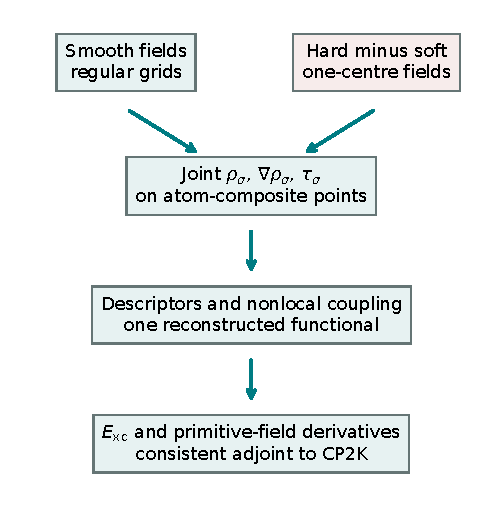
\includegraphics[width=\columnwidth]{native-reconstruction.pdf}
 \caption{The native implementation reconstructs the primitive fields before descriptor formation and Skala evaluation. The reverse operation follows the adjoint of the same reconstruction, preserving the hard-minus-soft signs. The atom-centred quadrature resolves local structure without requiring a uniformly fine regular grid.}
 \label{fig:reconstruction}
\end{figure}

\subsection{Accurate one-centre integration and joint reconstruction}

The accurate XC integration scheme in conventional GAPW improves cancellation between smooth-grid and soft atom-centred integrals evaluated on different quadratures.\cite{CP2K2020} The scheme uses the atom-local switch
\begin{equation}
 s_A(\mathbf r)=\exp[-\alpha_A|\mathbf r-\mathbf R_A|^2],
 \label{eq:xc-switch}
\end{equation}
where $\mathbf R_A$ is the nuclear position and $\alpha_A>0$ controls the inverse squared decay length of the dimensionless switch $s_A$. With periodic images implicit, the local or semilocal XC energy can be written schematically as
\begin{align}
 E_{\rm xc}^{\rm acc}\simeq{}&\int\!\left(1-\sum_A s_A\right)
                         e_{\rm xc}[\widetilde{\uvec}]\,d\mathbf r\nonumber\\
 &+\sum_A\int\!\left\{e_{\rm xc}[\uvec_A^h]
                  -(1-s_A)e_{\rm xc}[\uvec_A^s]\right\}d\mathbf r.
 \label{eq:accurate-integration}
\end{align}
Here, $e_{\rm xc}$ is a pointwise energy density, not an independent nonlocal Skala calculation, and $E_{\rm xc}^{\rm acc}$ denotes the energy in the accurate-integration scheme. Near a nucleus, the hard atom-centred term $e_{\rm xc}[\uvec_A^h]$ carries the rapidly varying contribution, while the nearly cancelling smooth and soft terms involving $\widetilde{\uvec}$ and $\uvec_A^s$ are suppressed. This rearrangement relies on GAPW's local matching assumptions. The switching weights $s_A$, quadrature, and their geometric derivatives must remain consistent.

Equation~\eqref{eq:accurate-integration} does not supply the mixed descriptors missing from Eq.~\eqref{eq:wrong}. The native Skala term instead uses its own jointly reconstructed fields and atom-composite quadrature. We retain accurate integration for the applicable conventional GAPW terms, but do not multiply the Skala reconstruction by the corresponding switching weights or add separately evaluated hard/soft Skala energies to it. This distinction separates an improvement of GAPW integration from the extension required for a learned nonlocal functional.

\subsection{Periodic atom-composite quadrature}

For a radial--angular point $\mathbf r_{Ai}$ centred on atom $A$, the discrete reconstruction is
\begin{equation}
 \begin{aligned}
 \uvec_{Ai,\sigma}={}&\sum_g I_{Ai,g}\widetilde{\uvec}_{g,\sigma}\\
 &+\sum_{B,\mathbf L}\left[\uvec^h_{B\mathbf L,\sigma}(\mathbf r_{Ai})
                        -\uvec^s_{B\mathbf L,\sigma}(\mathbf r_{Ai})\right].
 \end{aligned}
 \label{eq:composite}
\end{equation}
The interpolation $I$ maps the regular-grid fields to the target atom grid, with $I_{Ai,g}$ connecting regular-grid point $g$ to point $i$ of atom block $A$. The second sum includes neighbouring centres $B$ and periodic images $\mathbf L$, not only the target atom. Thus, ``one-centre'' describes the source expansion. It does not mean that its contribution is confined to a separate model call or omitted from neighbouring descriptor blocks. The sum is absent for direct-valence PP kinds, while intrinsic AE contributions are retained.

Let $w_{Ai}$ denote the unpartitioned radial--angular quadrature weight. Smooth atom-image partition functions define the energy weights through
\begin{equation}
 p_{A\mathbf L}(\mathbf r)=
 \frac{q_{A\mathbf L}(\mathbf r)}{\sum_{B,\mathbf L'}q_{B\mathbf L'}(\mathbf r)},
 \qquad \sum_{A,\mathbf L}p_{A\mathbf L}(\mathbf r)=1,
 \label{eq:partition}
\end{equation}
so that a target grid carries $W_{Ai}=w_{Ai}p_{A\mathbf0}(\mathbf r_{Ai})$, where $\mathbf0$ selects the central image of atom $A$. The differentiable shape functions $q$ provide a Becke-like partition.\cite{Becke1988} Periodic images distribute the integration over equivalent cells without double counting.

For the nonlocal descriptors, the partition is rebuilt using only the images $\mathcal S_A$ of the target atom $A$, giving
\begin{equation}
 \begin{aligned}
 d_A(\mathbf r)&=\frac{q^{\mathcal S_A}_{A\mathbf0}(\mathbf r)}
 {\sum_{(A,\mathbf L)\in\mathcal S_A}q^{\mathcal S_A}_{A\mathbf L}(\mathbf r)},\\
 D_{Ai}&=w_{Ai}\,T\!\left[d_A(\mathbf r_{Ai})\right].
 \end{aligned}
 \label{eq:descriptor-weights}
\end{equation}
The superscript identifies the centres used to construct the shape functions. The descriptor partition $d_A$ is not obtained by merely renormalizing the all-atom weights $p$. The smooth window $T$ suppresses negligible self-image weights and is unity away from that tail. Thus, $W_{Ai}$ weights the energy integral, whereas $D_{Ai}$ weights the model's internal nonlocal processing. An atom block sees the jointly reconstructed fields, including neighbouring atoms and their required images, throughout its windowed radial--angular grid. Neighbouring atoms affect these fields but do not partition the descriptor domain into separate atomic regions. The image sums are evaluated on finite target-block layouts. Normalization within a finite layout does not establish image-shell convergence. ESI Sec.~\ref{esi-sec:periodic-weights} defines the shape functions, window, image layouts, and interpolation. The geometric derivatives include the dependence on both sets of weights.

The role of $D_{Ai}$ can be made explicit by writing one nonlocal layer schematically as\cite{Skala2025}
\begin{equation}
 \begin{aligned}
 \mathbf m_A&=\sum_i D_{Ai}\,
     \mathsf K_\theta(\mathbf r_{Ai}-\mathbf R_A)\,\mathbf h_{Ai},\\
 \mathbf h'_{Ai}&=\mathcal U_\theta\!\left(
     \mathbf h_{Ai},\mathbf r_{Ai}-\mathbf R_A,\mathbf m_A\right).
 \end{aligned}
 \label{eq:nonlocal-layer}
\end{equation}
Here, $\mathbf h_{Ai}$ denotes transformed field features, or hidden features in later layers. The vector $\mathbf m_A$ collects their coarse atom-centred representation, and $\mathbf h'_{Ai}$ denotes the updated fine-grid features, with the prime indicating a layer update rather than a derivative. The kernel $\mathsf K_\theta$ comprises radial functions, spherical harmonics, and channel projections onto the atom-centred coarse point. The update $\mathcal U_\theta$ represents equivariant mixing and nonlinear contraction of the coarse features, their projection back onto the same atom's fine grid, and a local update. Repeating these layers yields the enhancement factor in Eq.~\eqref{eq:skala-energy}. The final energy uses $W_{Ai}$, not $D_{Ai}$. This schematic does not introduce message passing between different atomic coarse points. Neighbour information instead enters through the jointly reconstructed fields sampled by each block. The window therefore defines a nonlocal integration domain, not an isolated-atom density approximation.

The same construction reduces to a molecular atom-composite quadrature when no periodic images are required. A regular common grid can also support joint reconstruction, but resolving hard local fields everywhere is expensive. On the atom-composite grid, radial and angular resolution control the local structure independently of the plane-wave cutoff for the smooth contribution. This is an efficiency distinction, not a reason to evaluate different functionals on the two layouts.

Particle number provides an additional consistency check. The number of explicitly treated electrons is obtained from the density and overlap matrices as
\begin{equation}
 N=\sum_{\mathbf k\sigma}w_{\mathbf k}
           \mathrm{Tr}[P^\sigma(\mathbf k)S(\mathbf k)].
 \label{eq:particle-number}
\end{equation}
Here, $S(\mathbf k)$ is the Bloch-basis overlap matrix and $\mathrm{Tr}$ denotes the matrix trace. Integrating the reconstructed density gives $\widetilde N+\sum_A(N_A^h-N_A^s)$, where $\widetilde N$ and $N_A^{h,s}$ are the spin-summed integrals of the smooth and local hard/soft densities. The finite model quadrature instead gives $N_Q=\sum_{Ai\sigma}W_{Ai}\rho_{Ai,\sigma}$. A discrepancy between $N_Q$ and Eq.~\eqref{eq:particle-number} tests the field representation and quadrature. It does not, by itself, imply a change in the self-consistent-field (SCF) occupations. No density-dependent renormalization is applied, since it would alter both the functional and its variational derivative. Cutoff, radial/angular, and one-centre convergence are consequently distinct from changing the core treatment.

Finally, a nonlinear core correction (NLCC) must not be confused with hard-minus-soft reconstruction. An NLCC potential supplies a separate frozen-core density that can be added to the valence density and gradient before descriptor formation.\cite{Louie1982NLCC,Willand2013NLCC} It does not by itself provide a corresponding core kinetic-energy density. This is not equivalent to the explicit core orbitals of GAPW-AE, and it is not the origin of the one-centre corrections compared here.

\subsection{Variational coupling, forces, and stress}
\label{sec:variational}

Let $\mathcal R$ denote the discrete reconstruction from the density matrix $P$ to the model fields. The XC contribution to the generalized Kohn--Sham matrix is obtained by the chain rule as
\begin{equation}
 V_{\rm xc}=\left(\frac{\partial\mathcal R}{\partial P}\right)^{\!*}
             \frac{\partial E_{\rm xc}}{\partial\uvec}.
 \label{eq:adjoint}
\end{equation}
The asterisk denotes the adjoint under the chosen discrete contractions. The symbols $P$, $\uvec$, and $V_{\rm xc}$ collect the density matrices, model fields, and XC potential matrices, with spin indices implicit and k-point indices suppressed on the matrices. Overbars denote energy derivatives with respect to the indicated fields or local density-matrix coefficients. With $\overline{\uvec}_{Ai}=\partial E_{\rm xc}/\partial\uvec_{Ai}$, the component-wise adjoints from Eq.~\eqref{eq:composite} are
\begin{align}
 \overline{\widetilde{\uvec}}_g&=\sum_{Ai}I_{Ai,g}\overline{\uvec}_{Ai},\nonumber\\
 \overline D^h_A&=\left(\frac{\partial\uvec^h_A}{\partial D^h_A}\right)^{\!*}
                       \overline{\uvec},\qquad
 \overline D^s_A=-\left(\frac{\partial\uvec^s_A}{\partial D^s_A}\right)^{\!*}
                       \overline{\uvec}.
 \label{eq:component-adjoints}
\end{align}
The contractions include every target point to which a source contributes. The quadrature weights are already included in $\overline{\uvec}$, so applying them a second time would be incorrect. The local coefficients are then projected back to the orbital density matrix. Thus, the reverse path is the transpose of the actual discrete forward map, rather than an independently interpolated potential. This consistency is particularly important for the cancellation of hard and soft contributions and for SCF convergence near the numerical noise floor.
Kernel-level scalar-product tests verify the adjoint identity for the atom-local field interpolation, while equivalent back-projection variants agree at floating-point precision (ESI Table~\ref{esi-tab:adjoint-validation}). These checks complement the self-consistent force and stress tests below.

More explicitly, write the field adjoints as
\begin{equation}
 \begin{aligned}
 a_{Ai\sigma}&=\frac{\partial E_{\rm xc}}{\partial\rho_{Ai\sigma}},\qquad
 \mathbf b_{Ai\sigma}=\frac{\partial E_{\rm xc}}{\partial\nabla\rho_{Ai\sigma}},\\
 c_{Ai\sigma}&=\frac{\partial E_{\rm xc}}{\partial\tau_{Ai\sigma}}.
 \end{aligned}
 \label{eq:field-adjoints}
\end{equation}
Skala supplies the field derivatives through LibTorch automatic differentiation, while CP2K performs the adjoint reconstruction and assembles the XC matrix. These derivatives are obtained by back-propagating through all nonlocal layers and spin-gradient invariants of the full discrete energy, rather than differentiating an isolated local energy density. At fixed geometry, define the discrete field-response kernels $B^\rho$, $\mathbf B^g$, and $B^\tau$ for the density, its gradient, and the kinetic-energy density, respectively, by
\begin{equation}
 \delta\uvec_{Ai\sigma}=\sum_{\mathbf k\mu\nu}w_{\mathbf k}
 \begin{pmatrix}B^\rho_{Ai,\mu\nu}(\mathbf k)\\
 \mathbf B^g_{Ai,\mu\nu}(\mathbf k)\\B^\tau_{Ai,\mu\nu}(\mathbf k)\end{pmatrix}
 \delta P^\sigma_{\nu\mu}(\mathbf k).
 \label{eq:field-response}
\end{equation}
The symbol $\delta$ denotes a first-order variation at fixed geometry. With the convention $\delta E_{\rm xc}=\sum_{\mathbf k\sigma}w_{\mathbf k}
\mathrm{Tr}[V^\sigma_{\rm xc}(\mathbf k)\delta P^\sigma(\mathbf k)]$, the matrix is
\begin{equation}
 \begin{aligned}
 \bigl[V^\sigma_{\rm xc}(\mathbf k)\bigr]_{\mu\nu}
 &=\sum_{Ai}a_{Ai\sigma}B^\rho_{Ai,\mu\nu}(\mathbf k)\\
 &\quad+\sum_{Ai}\mathbf b_{Ai\sigma}\!\cdot\!\mathbf B^g_{Ai,\mu\nu}(\mathbf k)\\
 &\quad+\sum_{Ai}c_{Ai\sigma}B^\tau_{Ai,\mu\nu}(\mathbf k).
 \end{aligned}
 \label{eq:explicit-xc-matrix}
\end{equation}
For direct evaluation of orbital fields, these kernels would be
\begin{equation}
 \begin{aligned}
 B^\rho_{\mu\nu}&=\chi_{\mu\mathbf k}^*\chi_{\nu\mathbf k},\\
 \mathbf B^g_{\mu\nu}&=\nabla(\chi_{\mu\mathbf k}^*\chi_{\nu\mathbf k}),\\
 B^\tau_{\mu\nu}&=\tfrac12\nabla\chi_{\mu\mathbf k}^*\!\cdot\!\nabla\chi_{\nu\mathbf k},
 \end{aligned}
 \label{eq:orbital-field-kernels}
\end{equation}
evaluated at the target point $\mathbf r_{Ai}$. In the native GAPW implementation, however, the kernels in Eq.~\eqref{eq:field-response} include the smooth-grid interpolation, hard-minus-soft fields, and one-centre density-matrix projections of the actual reconstruction. Replacing them by direct orbital products would generally change the finite discretization. The real one-centre products and their derivatives are given in Eq.~\eqref{eq:one-centre-fields}. Equation~\eqref{eq:explicit-xc-matrix} adds no second quadrature factor or k-point weight. Its kinetic-energy-density term is a generalized Kohn--Sham matrix contribution rather than a multiplicative density potential.

At fixed orbital density matrix, the explicit XC derivative with respect to a nuclear coordinate or cell-strain parameter $\lambda$ includes geometry-dependent mappings and takes the form
\begin{equation}
 \left.\frac{\partial E_{\rm xc}}{\partial\lambda}\right|_P=
 \sum_{Ai}\overline{\uvec}_{Ai}\!\cdot\!
                 \left.\frac{\partial\uvec_{Ai}}{\partial\lambda}\right|_P
 +\left.\frac{\partial E_{\rm xc}}{\partial\lambda}\right|_{\uvec}.
 \label{eq:geometric-derivative}
\end{equation}
The restrictions $|_P$ and $|_{\uvec}$ hold the density matrix and model fields fixed, respectively, and the dot product contracts the field components and spin channels. The first term includes interpolation and hard/soft-field derivatives, while the second includes explicit model-coordinate and quadrature-weight dependence, including both periodic partitions. Stationarity of the complete electronic energy and the basis/overlap Pulay terms are then used to obtain the total force and stress. Because the XC contribution alone is not stationary with respect to the density matrix, model differentiation does not provide the full derivative of the self-consistent total energy. The nuclear force is $-dE/d\mathbf R_A$, and the strain derivative per cell volume gives the stress in the adopted sign convention. Self-consistent finite-difference (FD) checks of a force and diagonal stress component in a periodic water test support the derivative consistency of all five representations. Across the five tested representations and both FD step sizes, the maximum absolute discrepancies are approximately $2.9\times10^{-6}$~$E_h$/bohr and $4.7\times10^{-4}$~GPa. These results concern one Cartesian force component and one diagonal stress component of the periodic $\Gamma$-point water system. The FD protocol, numerical errors, and tested scope are documented in ESI Sec.~\ref{esi-sec:fd} and Table~\ref{esi-tab:derivatives}.

\subsection{K-points, symmetry reduction and parallelism}
\label{sec:kpoints}

Brillouin-zone integration on regular k-point meshes\cite{Monkhorst1976} enters through the density matrix and Eq.~\eqref{eq:rho}. Symmetry reduction must transform orbital components and Bloch phases consistently, together with the integration weights. Multiplying a scalar result by a symmetry count is insufficient. Once the real primitive fields are assembled, Skala need not know whether they originated from a full k-point mesh or a symmetry-reduced one. Their adjoints are returned to the corresponding complex Hermitian Kohn--Sham matrices. The native implementation uses CP2K's k-point and symmetry infrastructure,\cite{CP2KDynamics2026,Alizadeh2026PeriodicGFN2} with full point-group reduction through spglib in the molecular-crystal calculations.\cite{Togo2024Spglib} Numerical full/reduced-mesh comparisons are given in ESI Sec.~\ref{esi-sec:symmetry-meshes} and Table~\ref{esi-tab:symmetry}.

CP2K supplies fields, atom-associated coordinates, energy weights, and descriptor weights directly to the same Skala TorchScript model used by the molecular implementation. LibTorch returns the energy and input derivatives without a GauXC integration step. Complete atom blocks can be distributed over Message Passing Interface (MPI) ranks or batched on a device because the nonlocal processing retains the atom-block structure. Threaded field construction and back-projection complement inference on central processing units (CPUs) or graphics processing units (GPUs). Batching preserves the functional only if each block's descriptor domain and all contributing reconstructed fields are retained. This provides parallel execution without reverting to the separated smooth/hard/soft functional in Eq.~\eqref{eq:wrong}.

\section{Computational Strategy and Numerical Validation}
\label{sec:strategy}

We use the Skala-1.1 model distributed through Hugging Face\cite{SkalaModelCard} with its accompanying D3(BJ) dispersion contribution.\cite{Skala2025,Grimme2011D3BJ} We report the mean absolute error (MAE) and complementary error statistics, retaining each source's recorded dispersion contribution. The native Gaussian basis sets and GTH pseudopotentials use the 2026.2 parameter definitions of the University of Zurich (UZH) protocol.\cite{Mirhosseini2026UZH} The UZH AE bases are def2-derived bases optimized for GAPW using the molecularly optimized (MOLOPT) strategy, rather than unchanged def2 sets.\cite{Weigend2005,VandeVondele2007,Mirhosseini2026UZH} The native AE calculations use the triple- and quadruple-zeta valence plus double-polarization bases TZVPP-ae and QZVPP-ae, respectively, rather than the def2-TZVP/ma-def2-TZVP protocol of the earlier molecular GauXC study.\cite{Poeschel2026MolecularSkala} Bases with the same nominal zeta level can differ in accuracy between these families.

The molecular AE series for the dietGMTKN55 subset and the AE calculations for CO$_2$, NH$_3$, and urea treat every atom all-electron, as do the ICE13 crystals and their isolated-water references. The molecular and molecular-crystal comparisons also include calculations using GTH pseudopotentials for all atoms. Mixed AE/GTH calculations serve as additional core-treatment controls in LC10 and extend the band-gap study to compounds not fully covered by the available AE bases.

The numerical tests below guide the choice of settings for the molecular and condensed-phase applications presented in Sec.~\ref{sec:results}. For isolated molecules, each cell dimension is the corresponding molecular extent plus 25~\AA{}. We use nonperiodic boundary conditions and an analytic isolated-system Poisson solver, which evaluates an analytical reciprocal-space Green's function for zero-dimensional electrostatics using a truncated Coulomb kernel instead of the fully periodic one. Thus, molecular isolation does not rely on vacuum separation alone. The cell-padding study in ESI Sec.~\ref{esi-sec:padding} compares added extents of 22, 24, and 25~\AA{} under the same isolated-system electrostatics. These checks support the selected 25~\AA{} padding for our high-accuracy molecular calculations.

The regular-grid cutoff tests in ESI Sec.~\ref{esi-sec:cutoff} start with GAPW-AE for H$_2$O using the QZVPP-ae basis and a fixed 50/50 atom grid (Table~\ref{esi-tab:ae-cutoff}). Relative to the 1200~Ry reference, the total-energy deviations are substantially smaller at 600--1000~Ry than at 400~Ry. On this basis, we choose 640~Ry for the molecular AE calculations, which is slightly above the 600~Ry test point.

For GTH pseudopotentials, we compare the GPW and GAPW-XC alkane ACONF conformational energies, calculated with the TZV2P-GTH basis, against their respective 800~Ry results. The weaker cutoff dependence of GAPW-XC supports the choice of 400~Ry for the molecular GAPW-XC/GTH calculations (ESI Table~\ref{esi-tab:aconf-cutoff}). GTH pseudopotentials remove the explicit core electrons and smooth the valence orbitals, reducing the regular-grid resolution requirements. GAPW-XC further lowers these requirements by treating rapidly varying local contributions on atom-centred grids. At 800~Ry, the GPW and GAPW-XC conformational energies agree to within 0.009~kJ~mol$^{-1}$, supporting the accuracy of the combined GAPW density-decomposition and one-centre reconstruction approximations within GAPW-XC.

The plane-wave cutoff sets the resolution of the finest density grid, whereas the relative cutoff controls the assignment of Gaussian products to the multigrid levels. Increasing the latter assigns more products to finer grids. The higher AE cutoff is a conservative choice. GAPW treats the rapidly varying near-core density on atom-centred grids, but tighter Gaussian exponents retained in its smooth density representation can lead to slower plane-wave cutoff convergence.\cite{CP2KMadeSimple2026}

ESI Sec.~\ref{esi-sec:quadrature} independently tests radial and angular quadrature for GPW/GTH water at 800/60~Ry (Table~\ref{esi-tab:water-quadrature}). These tests show that increasing angular sampling alone is insufficient. Both radial and angular sampling must be refined to reduce the Skala quadrature error. Although the self-consistent density matrix has the prescribed electron number, fixed by its occupations and overlap-matrix trace, the finite atom-centred quadrature can still produce a different integral. We therefore monitor the integrated electron count separately to assess quadrature accuracy, without renormalizing the density.

Orbital-basis flexibility and integration accuracy are separate requirements. An AE basis must represent compact core states as well as the valence orbitals, whereas GTH pseudopotentials remove the explicit core states and smooth the valence orbitals. The molecular and lattice-energy comparisons motivate QZVPP-ae as the preferred AE basis for these energy studies, with the TZVPP-ae basis retained to quantify basis sensitivity (ESI Tables~\ref{esi-tab:urea-basis}, \ref{esi-tab:common62-summary}, and \ref{esi-tab:ice-basis}--\ref{esi-tab:ice-relative}). GTH calculations instead use the smaller valence-only TZV2P-GTH basis.



For lattice energies, numerical integration errors in the crystal and gas-phase molecular energies need not cancel. We therefore use the same refined integration settings for both phases. Crystal and molecule also use the same orbital basis, with isolated-system electrostatics for the gas-phase reference.

 In the molecular-crystal tests, the finer AE atom quadrature resolves the more rapidly varying core-density structure, while the smoother GTH valence density permits the less demanding quadrature used here. This local integration requirement is distinct from the choice of orbital basis and plane-wave cutoff.  The AE basis and quadrature comparisons are reported in ESI Sec.~\ref{esi-sec:crystal-numerical-controls}, Table~\ref{esi-tab:urea-basis}.



For the molecular crystals, the tested atom-centred quadrature refinement changes the lattice energy more than the tested k-point and symmetry-tolerance adjustments. CPU/CUDA lattice-energy differences are below 0.001~kJ~mol$^{-1}$ for CO$_2$ with GAPW-XC/GTH and urea with GAPW-AE. These controls and the crystal-only cutoff test are listed in ESI Table~\ref{esi-tab:x23_controls_si}. These fixed-input comparisons test device consistency. Full/reduced-mesh checks assess symmetry reduction at fixed k-point sampling (ESI Sec.~\ref{esi-sec:symmetry-meshes}), while self-consistent FD tests assess forces and stress (ESI Sec.~\ref{esi-sec:fd}).


OpenAI ChatGPT/Codex (GPT-5.6 Sol) assisted with the development of data-analysis and plotting scripts and with consistency checks during preparation of this work.

\section{Results and Discussion}
\label{sec:results}

\subsection{Molecular energetics and the GauXC connection}
\label{sec:molecular-results}

We use a selected set of 62 dietGMTKN55 reactions\cite{Gould2018,Goerigk2017} to test whether the periodic native-grid Skala implementation retains the molecular benchmark accuracy of our earlier molecular GauXC implementation in the isolated-molecule limit.\cite{Poeschel2026MolecularSkala} Each molecule is placed in a large supercell with nonperiodic boundary conditions and isolated-system electrostatics. On the same reactions, we compare GauXC GPW/GTH, GauXC GAPW-AE, native GAPW-XC/GTH, native GAPW-AE with the TZVPP-ae basis, and native GAPW-AE with the QZVPP-ae basis. PySCF provides an additional independent all-electron Skala comparison using the same def2-TZVP/ma-def2-TZVP basis protocol as GauXC GAPW-AE. %It is an implementation comparator, not the source of the dietGMTKN55 reference energies.

 The production settings follow the numerical tests in Sec.~\ref{sec:strategy} and are specified in ESI Sec.~\ref{esi-sec:molecular-data}.

The 62-reaction set was selected to ensure fully all-electron treatment of every constituent species in all four AE protocols. The two pure-GTH protocols are evaluated on this identical reaction set. %The selection is also guided by SCF convergence and the consistent availability of data across the earlier and present calculations, including internally consistent basis coverage within each protocol.

Table~\ref{tab:molecular-errors} summarizes the reference-error statistics for this common reaction set. Native QZVPP-ae, GauXC-AE, and PySCF give closely comparable mean absolute errors against the benchmark references. Native GAPW-XC/GTH and GauXC GPW/GTH show similarly good agreement in this measure. The mean absolute differences (MADs) between the corresponding native and GauXC reaction energies are reported separately in ESI Table~\ref{esi-tab:common62-pairs}. These MADs measure agreement between predictions, whereas the MAEs measure accuracy against the benchmark references. Complete statistics and reaction energies appear in ESI Tables~\ref{esi-tab:common62-summary}--\ref{esi-tab:common62-external}.


\begin{table}[tb]
\centering\small
\setlength{\tabcolsep}{3pt}
\caption{Unweighted mean absolute errors (MAEs) and root-mean-square errors (RMSEs) against the references for the same selected 62 dietGMTKN55 reactions, in kJ~mol$^{-1}$. The def2 entries use def2-TZVP/ma-def2-TZVP. The GTH entries use pseudopotentials.}
\label{tab:molecular-errors}
\begin{tabular}{@{}llrr@{}}
\toprule
Protocol & Basis & MAE & RMSE \\
\midrule
GauXC GAPW-AE & def2 & 4.05 & 9.94 \\
PySCF AE & def2 & 4.02 & 9.92 \\
Native GAPW-AE & TZVPP-ae & 7.14 & 14.72 \\
Native GAPW-AE & QZVPP-ae & 4.29 & 11.19 \\
\midrule
GauXC GPW/GTH & TZVP-GTH & 4.98 & 9.62 \\
Native GAPW-XC/GTH & TZV2P-GTH & 5.07 & 10.12 \\
\bottomrule
\end{tabular}
\end{table}


The slightly larger errors of the GTH protocols relative to the QZVPP-ae and def2 AE protocols are consistent with the trend reported in our molecular GauXC study.\cite{Poeschel2026MolecularSkala} In both GTH approaches, Skala receives the valence pseudodensity, without the explicit core-electron density and with a smoothed near-nuclear valence profile. This change from the AE training densities for light elements provides a plausible explanation for the trend. One-centre reconstruction of GTH valence fields does not recover the removed core electrons.

The effect of the native AE basis change on each reaction, including both improvements and deteriorations, is shown in ESI Fig.~\ref{esi-fig:common62-basis-improvements}.

The nominal triple-zeta def2-TZVP/ma-def2-TZVP protocol gives lower reference errors than TZVPP-ae on this selected set. However, with the QZVPP-ae basis, the native mean absolute error approaches those of GauXC and PySCF.

\subsection{Three molecular crystals with complementary bonding}
\label{sec:crystal-results}

CO$_2$, NH$_3$, and urea provide a compact test of transfer from isolated molecules to crystals. In nonpolar CO$_2$, cohesion combines London dispersion with electrostatic interactions between molecular quadrupoles, without hydrogen bonds. Polar NH$_3$ molecules form a network of directional N--H$\cdots$N hydrogen bonds. In urea, the carbonyl oxygen accepts hydrogen bonds from neighbouring N--H groups, connecting the polar molecules through an extended N--H$\cdots$O network.\cite{Morrison2003HydrogenBonds} The selection therefore contrasts dispersion-dominated binding with hydrogen-bonded environments that differ in donor--acceptor chemistry and network connectivity.

Crystal and independently supplied gas-phase molecular geometries are taken from the versioned supporting dataset of Della Pia \emph{et al.}\cite{DellaPia2024X23} We compare the electronic lattice energies with the corresponding diffusion Monte Carlo (DMC) references. For a unit cell containing $Z$ molecules, the lattice energy per molecule is
\begin{equation}
 E_{\rm latt}=E_{\rm crystal}/Z-E_{\rm molecule},
 \label{eq:lattice}
\end{equation}
where $E_{\rm crystal}$ is the total energy of the unit cell and $E_{\rm molecule}$ that of the isolated molecule, with negative values denoting binding. The comparison concerns electronic energies without thermal or zero-point contributions.

 The AE and GTH calculations use the QZVPP-ae and TZV2P-GTH bases, respectively. The full numerical protocol is specified in ESI Sec.~\ref{esi-sec:crystal-protocol}.

\begin{table*}[t]
\centering
\caption{Electronic lattice energies and MAEs against DMC for the same three crystals, in kJ~mol$^{-1}$ per molecule. The first four methods use native Skala--D3(BJ) with QZVPP-ae or TZV2P-GTH bases. Negative energies denote binding. Parentheses give DMC statistical uncertainties. The literature methods use different geometries and numerical protocols, detailed in ESI Sec.~\ref{esi-sec:crystal-literature}. Multi-level CCSD(T) denotes the composite LNO-CCSD(T)/RPA+ph/HF method.}
\label{tab:crystals}
\begin{tabular}{lrrrr}
\toprule
Method & CO$_2$ & NH$_3$ & Urea & MAE\\
\midrule
GAPW-AE & -32.067 & -38.185 & -110.427 & 1.54\\
GAPW-GTH one-centre & -37.392 & -40.076 & -113.719 & 5.03\\
GAPW-GTH direct & -37.376 & -40.094 & -113.805 & 5.06\\
GAPW-XC/GTH & -37.408 & -40.074 & -113.725 & 5.04\\
\midrule
PBE+D3\cite{DellaPia2025MLIP} & -25.07 & -43.76 & -109.90 & 3.76\\
SCAN+rVV10\cite{DellaPia2025MLIP} & -31.47 & -41.69 & -113.55 & 3.54\\
PBE0+MBD\cite{DellaPia2025MLIP} & -23.74 & -38.99 & -109.40 & 2.45\\
MP2/CBS\cite{Liang2023CrystalMP2} & -27.81 & -38.34 & -108.66 & 0.63\\
Multi-level CCSD(T)\cite{Syty2025CrystalCC} & -29.4 & -37.6 & -111.0 & 1.03\\
\midrule
DMC reference\cite{DellaPia2024X23} & -29.4(2) & -38.2(1) & -108.5(3) & --\\
\bottomrule
\end{tabular}
\end{table*}

The comparison with DMC benchmarks the accuracy of each complete Skala--D3(BJ) protocol. Differences between AE and GTH reflect the combined effects of core treatment, orbital basis, and atom quadrature. In contrast, direct and one-centre GAPW-GTH retain the same pseudopotentials, basis, and integration settings, providing a targeted test of valence-field reconstruction.

The three GTH representations give stronger binding than DMC and agree closely with one another (Table~\ref{tab:crystals}). The direct and one-centre GTH lattice energies differ by less than 0.09~kJ~mol$^{-1}$, making the numerical effect of the one-centre approximation negligible on the scale of the deviations from DMC. In contrast, the larger-basis AE results approach the DMC references, with essentially zero residual for ammonia.

The QZVPP-ae calculations reduce the overbinding relative to GAPW-XC/GTH for all three crystals. Ammonia is the most accurate case, while CO$_2$ retains the largest absolute and fractional error in every representation. Enlarging both the crystal and molecular AE bases at fixed fine quadrature reduces the three-crystal MAE from 7.95 to 1.54~kJ~mol$^{-1}$.  For AE urea, the $+14.42$~kJ~mol$^{-1}$ shift from TZVPP-ae to QZVPP-ae at fixed 200/974 quadrature is much larger than the $-0.21$~kJ~mol$^{-1}$ shift from refining the quadrature from 150/770 to 200/974 with the TZVPP-ae basis. This identifies basis flexibility as the dominant tested contribution and motivates the larger AE basis independently of the integration-grid choice. Thus, the native implementation delivers highly accurate molecular-crystal energies when sufficient AE basis flexibility is supplied, without changing the functional, geometries, or one-centre reconstruction. The basis-set and integration-grid convergence tests and the DMC errors at both basis levels are documented in ESI Sec.~\ref{esi-sec:crystal-numerical-controls}, Tables~\ref{esi-tab:urea-basis} and \ref{esi-tab:crystal-basis-errors}.


The material-dependent errors may reflect different balances of intermolecular attraction, repulsion, and molecular deformation. Dispersion-dominated CO$_2$ tests a delicate balance of attractive correlation, quadrupolar electrostatics, and short-range repulsion. Earlier correlated calculations also find a larger gas-to-crystal intramolecular deformation contribution for urea.\cite{Sharkas2014Crystals}

For CO$_2$, excessive attraction or insufficient short-range repulsion could each produce the remaining overbinding. Its smaller reference lattice energy also amplifies the fractional error.  This contrasts with the consistently small NH$_3$ residual, which may involve favourable cancellation between crystal and molecular errors.

The tested integration-grid and CPU/GPU effects are too small to explain the remaining CO$_2$ discrepancy. The close agreement among the GTH representations also shows that the choice of density reconstruction has little influence on this residual.

We compare Skala--D3(BJ) electronic lattice energies with DMC references, avoiding the zero-point and thermal corrections required when using experimental sublimation enthalpies.\cite{DellaPia2024X23,Dolgonos2019X23b}


Table~\ref{tab:crystals} places the native results alongside selected dispersion-inclusive DFT and correlated wavefunction calculations. Native GAPW-AE has a lower MAE than the listed DFT methods, while GAPW-XC/GTH is competitive for ammonia and urea. MP2/CBS and the multi-level LNO-CCSD(T)/RPA+ph/HF approach give smaller MAEs than native AE, but the differences are on the scale of the estimated overall DMC uncertainty.\cite{DellaPia2024X23} The literature geometries and numerical protocols are documented in ESI Sec.~\ref{esi-sec:crystal-literature}.

\subsection{Ice polymorphs and condensed-phase transferability}
\label{sec:transfer-results}



The DMC-ICE13 calculations compare the TZVPP-ae and QZVPP-ae bases at fixed crystal geometries using the same integration settings at both basis levels. The full numerical protocol and gas-phase reference geometry are specified in ESI Sec.~\ref{esi-sec:ice-protocol}.

The complete DMC-ICE13 comparison provides a broader test of hydrogen-bonded condensed phases.\cite{DellaPia2022Ice} Across the thirteen phases calculated at both basis levels, enlarging the AE basis reduces the absolute lattice-energy MAE from 21.35 to 1.16~kJ~mol$^{-1}$.  The systematic TZVPP-ae overbinding is not retained with the QZVPP-ae basis. The MAE of the twelve energy differences relative to Ih also decreases, from 4.17 to 0.82~kJ~mol$^{-1}$. Figure~\ref{fig:ice13-errors} shows their deviations from DMC by phase. This comparison cancels the gas-phase reference exactly, showing that the improvement is not merely a common shift in binding. Nevertheless, QZVPP-ae underestimates eleven of these twelve relative energies, with the largest residual for VII.  Differences in the ordering of nearly degenerate phases also remain. ESI Sec.~\ref{esi-sec:ice-basis} and Tables~\ref{esi-tab:ice-basis} and \ref{esi-tab:ice-relative} give the phase-resolved comparison.

\begin{figure*}[t]
\centering
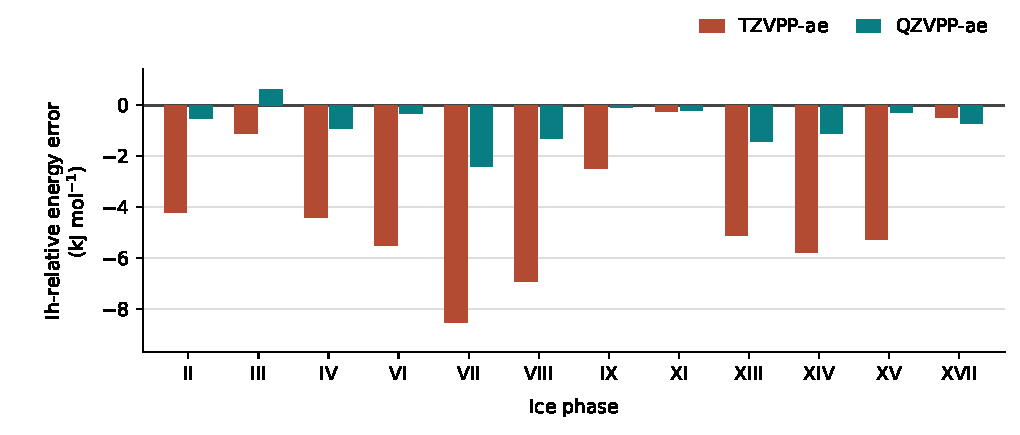
\includegraphics[width=\textwidth]{ice13-energy-errors.pdf}
\caption{Deviations of Ih-relative native Skala--D3(BJ) GAPW-AE energies from DMC-ICE13 references\cite{DellaPia2022Ice} for the TZVPP-ae and QZVPP-ae bases. The bars show $\Delta E_p-\Delta E_p^{\rm DMC}$ for the twelve phases other than Ih, where $\Delta E_p=E_{{\rm latt},p}-E_{{\rm latt},{\rm Ih}}$ is the lattice-energy difference per water molecule between phase $p$ and Ih. Negative deviations indicate underestimated energy differences. Full energies and DMC statistical uncertainties are given in ESI Tables~\ref{esi-tab:ice-basis} and \ref{esi-tab:ice-relative}.}
\label{fig:ice13-errors}
\end{figure*}

Taken together, the larger-basis molecular-crystal and ice results demonstrate accurate lattice energies across these condensed-phase environments.




\subsection{Equilibrium crystal structures}
\label{sec:structure-results}

The ten-solid equation-of-state comparison (LC10) probes equilibrium structures rather than energies at fixed reference geometries. All ten lattice constants lie below the static-lattice reference values in each of the four native representations, with MAEs of 0.073--0.084~\AA{} (Table~\ref{tab:lc10-primary} and ESI Table~\ref{esi-tab:lc10-reconstruction}). This systematic lattice contraction indicates structural overbinding, distinct from the accurate fixed-geometry molecular-crystal and ice lattice energies. The EOS results and numerical protocol are given in ESI Sec.~\ref{esi-sec:solids}. Enlarging the AE basis to QZVPP-ae reduces the diamond lattice error but increases the Si contraction, with a smaller change for MgO (ESI Sec.~\ref{esi-sec:solid-basis}).

\begin{table*}[t]
\centering\small
\caption{Equilibrium lattice constants $a_0$ and bulk moduli $B_0$ for the ten LC10 solids using GAPW-XC/GTH and GAPW-AE. Experimental static-lattice references follow Ref.~\citenum{Goldzak2022Solids}. Each MAE is calculated over all ten solids in the unit of the corresponding column.}
\label{tab:lc10-primary}
\begin{tabular}{lrrrrrr}
\toprule
& \multicolumn{3}{c}{$a_0$ (\AA{})} & \multicolumn{3}{c}{$B_0$ (GPa)} \\
\cmidrule(lr){2-4}\cmidrule(lr){5-7}
Solid & Experiment & \shortstack{GAPW-XC/\\GTH} & GAPW-AE & Experiment & \shortstack{GAPW-XC/\\GTH} & GAPW-AE \\
\midrule
AlN & 4.3680 & 4.2811 & 4.3025 & 206.00 & 239.07 & 225.89 \\
AlP & 5.4480 & 5.3622 & 5.3781 & 87.00 & 94.34 & 101.35 \\
BN & 3.5930 & 3.5777 & 3.5675 & 388.50 & 423.39 & 420.87 \\
BP & 4.5250 & 4.4439 & 4.4696 & 176.50 & 187.93 & 183.64 \\
C & 3.5530 & 3.5345 & 3.5292 & 453.30 & 457.33 & 491.35 \\
LiCl & 5.0720 & 4.9081 & 4.9155 & 37.30 & 47.98 & 46.37 \\
MgO & 4.1890 & 4.1059 & 4.0935 & 173.00 & 188.28 & 198.71 \\
MgS & 5.1880 & 5.0689 & 5.0536 & 81.00 & 87.90 & 90.27 \\
Si & 5.4210 & 5.3386 & 5.3740 & 100.30 & 92.76 & 100.56 \\
SiC & 4.3470 & 4.2517 & 4.2920 & 228.90 & 263.89 & 241.68 \\
\midrule
MAE & -- & 0.0831 & 0.0728 & -- & 16.61 & 16.89 \\
\bottomrule
\end{tabular}
\end{table*}

The pure-AE series has the smallest lattice-constant MAE, but every core-treatment protocol retains the contraction. At fixed element-wise core treatment, the direct and one-centre GAPW-AE/GTH variants give nearly identical equilibrium lattice constants. Across the five genuinely mixed and three all-GTH systems, their differences remain below $6\times10^{-4}$~\AA{}. The bulk moduli are more sensitive to the representation, particularly for MgO (ESI Table~\ref{esi-tab:lc10-reconstruction}). Thus, the GTH valence-reconstruction choice has little influence on the equilibrium lattice contraction, although the curvature of the energy--volume curve is more affected.

This structural bias should be considered in light of the training domain. Skala-1.1 was developed from molecular and atomic reference data rather than periodic-solid densities and energies.\cite{Skala2025,Ehlert2026ACC} Limited coverage of extended coordination, screening, and cooperative polarization is therefore a possible contributor to the LC10 contraction, alongside basis, core-treatment, and dispersion effects. High-accuracy periodic reference data are needed to assess these contributions and to guide a targeted extension or reparameterization of the XC functional.

High-accuracy reference data can be obtained with periodic wavefunction-based methods,\cite{Azadi2020Hydrogen} including periodic coupled-cluster theory\cite{Hummel2017,Gruber2018} and full configuration-interaction quantum Monte Carlo (FCIQMC).\cite{Booth2013} Complementary real-space quantum Monte Carlo (QMC) approaches use flexible trial wavefunctions based on shadow\cite{Calcavecchia2014Shadow,Calcavecchia2015Shadow,Calcavecchia2018} and resonating-valence-bond constructions,\cite{Azadi2015Ozone} or neural networks.\cite{Kessler2021,Hermann2020PauliNet,Pfau2020FermiNet}


\subsection{Electronic band gaps}
\label{sec:bandgap-results}

We assess Skala's electronic band gaps using triple-zeta GAPW-AE, GAPW-XC/GTH, and mixed AE/GTH one-centre calculations for the experimentally referenced materials considered by Lee \emph{et al.}\cite{Lee2021Gaps,Lee2022Hybrids}

To separate electronic-structure errors from geometry-induced shifts, the band-gap calculations use fixed experimental geometries rather than Skala-optimized structures, with a uniform triple-zeta protocol and fixed insulating occupations.  ESI Sec.~\ref{esi-sec:bandgap-protocol} records the phase-specific experimental geometries, basis sets, core choices, Brillouin-zone sampling, and convergence thresholds.

We report 50 band-gap results for 28 materials, comprising 20 AE, 23 GAPW-XC/GTH, and seven mixed one-centre results.

The combined AE-or-mixed one-centre series contains fifteen pure-AE and seven mixed results on 22 materials also available for GAPW-XC/GTH. The respective MAEs are 0.543 and 0.816~eV. Both native series have smaller MAEs than PBE, SCAN, and B97M-rV on exactly these 22 materials. ESI Tables~\ref{esi-tab:bandgap-outcomes} and \ref{esi-tab:bandgap-paired-combined-Lee2021} report the individual gaps, experimental references, and all ten local or semilocal comparators.

Fifteen of these materials also occur in the published hybrid-functional comparison, with twelve AE and three mixed native results. On this common population, the AE-or-mixed and GAPW-XC/GTH MAEs are 0.432 and 0.778~eV. Table~\ref{tab:bandgap-method-errors} compares the native results with all ten local or semilocal and twelve hybrid XC functionals on exactly these fifteen materials. The AE-or-mixed MAE is comparable to those of HSE, PBE0, and B3LYP, although its RMSE is larger. On the same fifteen-material set, its MAE is substantially lower than that of M06-2X and those of all four range-separated hybrid functionals included in the table. The ordering of the closely spaced Skala and HSE MAEs reverses when the BAs reference is changed from 1.46~eV to the independently reported 1.82~eV absorption estimate (ESI Table~\ref{esi-tab:bandgap-BAs-sensitivity}).\cite{Yue2020BAs}

\begin{table}[tb]
\centering\small
\setlength{\tabcolsep}{2.5pt}
\caption{Band-gap errors in eV for the fifteen materials common to the native calculations and both literature benchmarks.\cite{Lee2021Gaps,Lee2022Hybrids} Skala AE/mixed comprises twelve AE and three mixed AE/GTH one-centre results. Skala GTH denotes GAPW-XC/GTH. All ten local or semilocal and twelve hybrid XC comparators use the same set of BAs, BN, BP, C, CdS, CdSe, GaAs, GaP, Ge, InP, LiCl, Si, ZnS, ZnSe, $\beta$-GaN. ME is calculation minus experiment averaged over the set. mGGA denotes meta-GGA. RS denotes range separation. Individual gaps are given in ESI Table~\ref{esi-tab:bandgap-outcomes}.}
\label{tab:bandgap-method-errors}
\begin{tabular}{@{}llrrr@{}}
\toprule
Method & XC class & ME & MAE & RMSE \\
\midrule
Skala AE/mixed & Native & -0.365 & 0.432 & 0.602 \\
Skala GTH & Native & -0.776 & 0.778 & 0.926 \\
\midrule
LDA & LDA & -1.411 & 1.411 & 1.574 \\
PBE & GGA & -1.181 & 1.181 & 1.339 \\
PBEsol & GGA & -1.327 & 1.327 & 1.483 \\
revPBE & GGA & -1.097 & 1.097 & 1.249 \\
BLYP & GGA & -1.066 & 1.085 & 1.248 \\
B97-D & GGA & -1.026 & 1.043 & 1.180 \\
SCAN & mGGA & -0.947 & 0.961 & 1.086 \\
M06-L & mGGA & -0.793 & 0.845 & 1.010 \\
MN15-L & mGGA & -1.083 & 1.095 & 1.248 \\
B97M-rV & mGGA & -0.845 & 0.872 & 1.016 \\
\midrule
B3LYP & Hybrid GGA & +0.097 & 0.405 & 0.510 \\
PBE0 & Hybrid GGA & +0.285 & 0.402 & 0.502 \\
revPBE0 & Hybrid GGA & +0.355 & 0.451 & 0.521 \\
B97-3 & Hybrid GGA & +0.640 & 0.692 & 0.739 \\
M06-2X & Hybrid mGGA & +2.057 & 2.057 & 2.123 \\
MN15 & Hybrid mGGA & +0.894 & 0.931 & 1.080 \\
SCAN0 & Hybrid mGGA & +0.399 & 0.453 & 0.545 \\
HSE & Screened hybrid & -0.387 & 0.435 & 0.578 \\
CAM-B3LYP & RS hybrid & +2.411 & 2.411 & 2.453 \\
$\omega$B97X-rV & RS hybrid & +3.988 & 3.988 & 4.011 \\
$\omega$B97M-rV & RS hybrid & +3.492 & 3.492 & 3.528 \\
CAM-QTP01 & RS hybrid & +4.203 & 4.203 & 4.231 \\
\bottomrule
\end{tabular}
\end{table}


The mixed one-centre protocol reduces the gap underestimation relative to GAPW-XC/GTH on all seven compounds shared by these two series, lowering the MAE from 0.766 to 0.650~eV (ESI Table~\ref{esi-tab:bandgap-core-subsets}). This comparison includes changes in core treatment and the corresponding element-specific orbital bases. For Ge and MgS, the sampled gaps are indirect with GAPW-AE but direct with GAPW-XC/GTH, illustrating that the AE/GTH protocol affects not only the gap magnitude but also the relative positions of the band extrema (ESI Table~\ref{esi-tab:bandgap-edges}).

The separate direct/one-centre controls retain the AE reconstruction and test the GTH valence representation in six genuinely mixed compounds and one all-GTH control. The one-centre reconstruction of GTH valence fields changes the calculated gaps by less than 0.009~eV across the seven tested systems (ESI Table~\ref{esi-tab:bandgap-controls}).

\section{Conclusions}

The joint one-centre reconstruction brings learned nonlocal XC into CP2K's native GPW/GAPW framework without GauXC. Reconstructing density, gradients, and kinetic-energy density before evaluation preserves the mixed terms and nonlocal couplings required by GAPW-XC, GAPW-AE, and augmented GAPW-GTH. GAPW-XC is the recommended default starting representation for pseudopotential calculations because rapidly varying contributions to the XC input fields are resolved on atom-centred grids independently of the global plane-wave cutoff. The same variational construction connects the functional to CP2K's forces, stress, k-point sampling, and point-group reduction, and to its boundary-condition framework for systems of different dimensionality. The present validation covers molecules and three-dimensional crystals.

With the QZVPP-ae basis, native GAPW-AE reaches a molecular MAE close to that of our earlier def2-based GauXC implementation on the same selected set of 62 reactions from dietGMTKN55. At the nominal triple-zeta level, however, the def2 protocol has the more favourable error balance. The improvement with the larger AE basis identifies basis flexibility as an important source of the initial deviations. Together with the numerical consistency tests, these results show that the native implementation preserves Skala's molecular predictive accuracy while extending its application to condensed-phase electronic structure.

Skala with D3(BJ) achieves excellent agreement with DMC for the three molecular crystals when the AE basis is enlarged uniformly to QZVPP-ae. The resulting MAE is 1.54~kJ~mol$^{-1}$. The complete thirteen-phase ice comparison independently reaches MAEs of 1.16~kJ~mol$^{-1}$ for absolute lattice energies and 0.82~kJ~mol$^{-1}$ for the twelve relative energies to Ih. Residual phase-dependent errors and a bias towards underestimated relative energies remain. These results highlight the importance of basis flexibility when assessing the functional's condensed-phase accuracy. The triple-zeta GTH calculations give errors comparable to those of established dispersion-inclusive approximations for ammonia and urea. Together with the numerical controls, the molecular-crystal and ice results support both the native implementation and accurate transfer beyond the gas phase, while motivating broader condensed-phase validation with many-body references.

The band-gap calculations assess transferability to electronic structure at fixed experimental geometries. On the matched 22-material population, the preselected AE-or-mixed series has smaller mean absolute gap errors than PBE, SCAN, and B97M-rV. On the distinct fifteen-material set shared with the hybrid-functional study, its 0.432~eV MAE is comparable to those of HSE, PBE0, and B3LYP. These results complement the accurate molecular-crystal and ice energies at fixed geometries. In contrast, the systematically underestimated LC10 equilibrium lattice constants reveal a remaining structural bias.

Periodic coupled-cluster and QMC calculations, including FCIQMC where feasible, can supply the required many-body reference data. Reference energies and densities spanning periodic environments and volumes would allow us to test directly whether the molecular training data adequately cover condensed-phase environments. They would also provide a basis for targeted retraining or reparameterization of Skala aimed at reducing the remaining structural bias while preserving its molecular accuracy. The native GPW/GAPW implementation allows this development within the same electronic-structure framework used for subsequent applications.

\section*{Conflicts of interest}
% The authors confirmed that there are no conflicts of interest.
There are no conflicts to declare.

\section*{Data availability}
\label{sec:data-availability}
The supporting reaction energies, lattice-energy comparisons, equation-of-state data, band-gap tables, and numerical controls are included in the ESI. The underlying energies, geometries, computational inputs and outputs, reference data, analysis scripts, and source-version metadata for all benchmarks and numerical controls are publicly available at \url{https://github.com/DCM-Uni-Paderborn/native-grid-skala-benchmarks}. For the comparison with earlier molecular implementations, this repository contains the matched reference extract and links to the original molecular Skala repository rather than duplicating its full dataset.

\section*{Acknowledgements}
The authors thank the AI for Science team at Microsoft Research for valuable discussions and the CP2K and GauXC development communities. Part of the research was funded by the German Research Foundation (DFG), project numbers 417590517/Collaborative Research Centre 1415 and 519869949.

During the preparation of this work, the authors used OpenAI ChatGPT/Codex (GPT-5.6 Sol) to support language editing, literature organization, mathematical exposition, the development of data-analysis and plotting scripts, consistency checks, and LaTeX preparation. The authors reviewed and edited the resulting content and take full responsibility for the content of the published article.

\bibliographystyle{rsc}
\bibliography{references}
\end{document}
